\documentclass[12pt, a4paper]{article}

\usepackage[utf8]{inputenc}
\usepackage[russian]{babel}
\parindent 0pt
\parskip 8pt
\usepackage{amsmath}
\usepackage{amssymb}
\usepackage{array}
\usepackage{floatrow}
\usepackage{float}
\usepackage[left=2.3cm, right=2.3cm, top=2.7cm, bottom=2.7cm, bindingoffset=0cm]{geometry} % headheight=0pt,
\usepackage{hyperref}
\usepackage{graphicx}
\usepackage{multicol}
\usepackage{fancyhdr} 
\usepackage{extramarks}
\usepackage[usenames,dvipsnames]{color}
\usepackage{titlesec}
\usepackage{tikz}
\definecolor{grey}{RGB}{128,128,128}

\pagestyle{fancy}
\fancyhf{}
\lhead{Билет № 2.2}
\chead{Архитектура набора команд (ISA) и микроархитектура}
\rhead{\thepage}
\lfoot{made with Ы}
\cfoot{}
\rfoot{\today}
\renewcommand\headrulewidth{0.4pt}
\renewcommand\footrulewidth{0.4pt}

\titlespacing*{\section}{0pt}{5pt}{0pt}
\titlespacing*{\subsection}{0pt}{5pt}{0pt}
\titlespacing*{\subsubsection}{0pt}{5pt}{0pt}

\begin{document}
\section{ISA}
\textbf{ISA} - \textit{Instruction Set Architecture} - Архитектура Набора Команд.
\subsection{Немного истории}
Первой ISA была линейка компьютеров IBM под названием System/360. Это была линейка из четырех компьютеров с разной аппаратной частью, соотвественно с разной точностью вычислений, скоростью работы и ценой. Однако, любая программа написанная для простой модели могла запускаться на более сложных моделях линейки без внесения изменений, а также потенциально и любая программа для сложной машины могла выполняться на более простых. Т.е. набор команд для всех машин линейки был одинаков.
\subsection{Что такое ISA?}
ISA - некоторый документ, который описывает:
\begin{itemize}
    \item архитектуру памяти,
    \item набор команд, доступных программисту, пишущему на машинном языке,
    \item количество регистров,
    \item доступные типы данных,
    \item обработку исключений и прерываний (что происходит при делении на 0 и т.д.),
    \item разрядность адресов,
    \item протокол взаимодействия с внешними устройствами ввода/вывода,
    \item режимы адресации,
    \item разграничение доступа (привелигированный доступ для ОС, пользовательский для пользователя)
\end{itemize}
\subsection{Примеры ISA}
x86, x86\_64, ARM, MIPS, System/360 
\section{Архитектуры памяти}
\subsection{Стековая архитектура}
Набор команд by SKKV:
\begin{itemize}
    \item Арифметика: sub, add, mul, div (для вычитания и деления: первый операнд - то, что первым сняли со стека)
    \item Доп. арифметика: subr, divr (первый операнд - то, что сняли вторым со стека)
    \item Операции с памятью: push[a], pop[a]. a - адрес ячейки в RAM.
    \item Операции со стеком: pop - выкинуть верхнее значение, push StX - добавить на вершину стека копию ячейки с номером Х относительно вершины стека (вершина - St0, следующая за ней ячейка - St1 и т.д)
\end{itemize}
Взаимодействия в целом вида: снять два верхних значения со стека, произвести с ними операцию, положить результат обратно на стек.
\subsection{Аккумуляторная архитектура}
Можно определить как стек размера 1, или как регистровую архитектуру с одним регистром. Эта единственная ячейка называется аккумулятором. Работает очень медленно, зато просто и дешево производить\\
Набор команд by SKKV:
\begin{itemize}
    \item Работа с памятью: LD[a] - загрузить ячейку из памяти, ST[a] - положить ячейку в память. a - адрес ячейки в RAM
    \item Арифметические операции: mul a, sub a, add a, div a. a - адрес второго операнда в RAM. Первый операнд - значение, лежащее в аккумуляторе. Результат операции помещается в аккумулятор.
\end{itemize}
\subsection{Регистрово-регистровая архитектура, Reg-Reg}
Есть фиксированное число регистров R0, R1 ... RN. Итерировать по ним нельзя! Цифры - не индексы, а часть названия.\\
Есть две вариации Reg-Reg 2 - операторы принимают два операнда.\\
SUB R1 R2 ~~~ R1 -= R2\\
И Reg-Reg 3 - операторы принимают три операнда.\\
SUB R1 R2 R3 ~~~ R1 = R2 - R3\\
SUB R1 R1 R2 ~~~ R1 -= R2\\
Набор команд by SKKV:
\begin{itemize}
    \item Арифметика: SUB, ADD, MUL, DIV. Работают только с регистрами!! Константы допускаются на последнем месте (SUB R1 R1 5 или SUB R1 5).
    \item Операции с регистрами: MOV R1 R2 - скопировать значение регистра R2 в регистр R1.
    \item Операции с памятью: LD R1 [a] - загрузить в R1 значение по адресу a. ST [a] R0 - загрузить в ячейку по адресу [a] значение регистра R0.
\end{itemize}
\subsection{Reg-Mem архитектура}
Всё так же, как и в Reg-Reg, только один из операндов может быть адресом в памяти (а может и не быть, как напишешь).\\
В чем преимущество перед Reg-Reg: команды компактнее, следовательно больше команд влезет в кэш.\\
В чем недостаток: чуть медленнее, больше команд, сложнее реализовать.
\subsection{Mem-Mem}
Теперь все операнды могут быть ячейками в памяти. Использовалось в древних компьютерах.
\section{Кодирование команд}
Есть два стула:
\begin{enumerate}
    \item Команды переменной длины.\\
    Можем часто используемые команды сделать поменьше и выиграть с кэшированием. С другой стороны, такие команды сложнее декодировать.\\
    В х86 используются команды переменной длины 1..15 байт.
    \item Команды фиксированной длины.\\
    Теперь просто декодировать, но, например, загрузку 32х битной константы в 32х битный регистр придется разбить на две операции.\\
    В MIPS используются команды фиксированной длины в 4 байта.
\end{enumerate}
\section{RISC и CISC}
\subsection{CISC}
\textbf{CISC} - Complex Instruction Set Computer - много разных команд (в VAX, например, было 200-300).\\
Обычно reg-mem, обычно переменная длина команд.
\subsubsection{Преимущества}
\begin{itemize}
    \item быстрее выполняем всякие упопротые сложные команды, т.к. для них есть отдельные аппаратные вычислительные блоки
    \item лучше с энергоэффективностью
\end{itemize}
\subsubsection{Недостатки}
\begin{itemize}
    \item упоротые команды используются не так уж и часто, а вычислительные блоки занимают место 
\end{itemize}
\subsection{RISC}
\textbf{RISC} - Reduced Instruction Set Computer - мало команд.\\
Обычно reg-reg, обычно фиксированная длина команд.
\subsubsection{Преимущества}
\begin{itemize}
    \item можем поставить на кристалл больше простых вычислителей и выиграть по скорости за счет параллельности. или можем добавить на кристалл кэша
    \item быстрее
\end{itemize}
\subsubsection{Недостатки}
\begin{itemize}
    \item энергоэффективность. какое-нибудь программно реализованное шифрование диска быстро сожрало бы аккумулятор, а аппаратным блоком всё ок.
\end{itemize}
\subsection{В итоге}
x86 - CISC снаружи, там очень много всяких разных сложных команд, но аппаратно это RISC. Где-то есть небольшой блок, который преобразует CISC команды в RISC команды, которые затем исполняются.\\
Такой фокус необходим для сохранения обратной совместимости (в ISA можно добавить команд, а вот выкинуть нельзя).
\section{Режимы адресации\textasciicircum}
\begin{table}[h]
\begin{tabular}[width=\linewidth]{|c|c|c|}
     Register & ADD R4 R1 R2 & regs[R4] <- regs[R1] + regs[R2] \\
     Immediate & ADD R4 R1 5 & regs[R4] <- regs[R1] + 5\\
     Displacement & ADD R4 R1 100(R2) & regs[R4] <- regs[R1] + MEM[100 + regs[R2]]\\
     Register Indirect & ADD R4 R1 (R2) & regs[R4] <- regs[R1] + MEM[regs[R2]]\\
     Absolute & ADD R4 R1 [0x123] & regs[R4] <- regs[R1] + MEM[0x123]\\
     Memory Indirect & ADD R4 R1 @(R2) & regs[R4] <- regs[R1] + MEM[MEM[regs[R2]]]\\
     PC Relative & ADD R4 R1 100(PC) & regs[R4] <- regs[R1] + MEM[100 + PC]\\
     Scaled & ADD R4 R1 100(R1)[R5] & regs[R4]<-regs[R1] + MEM[100 + regs[R1] + regs[R5] * 4]
\end{tabular}
\end{table}
\begin{itemize}
    \item Register - Регистровая адресация. Операнды - данные, хранящиеся в регистре (ну на самом деле не совсем всё так, но упростим)
    \item Immediate - Непосредственная индексация. Хранение в адресной части самого операнда, а не его адреса. Так можно работать только с константами
    \item Displacement - Индексная адресация. Обращение к памяти по значению регистра и какому-то константному смещению.
    \item Register Indirect - Косвенная регистровая адресация - обращаемся к памяти по значению регистра
    \item Absolute - Абсолютная адресация. Обращение к памяти по константному адресу. В современных архитектурах почти не используется.
    \item Memory Indirect*** - Косвенная адресация к памяти(?). Обращаемся к ячейке памяти по значению, которое лежит в другой ячейки памяти, адрес которой лежит в регистре. Уххх. Используется, например, в VAX
    \item PC (IP) Relative* - Адресация относительно счетчика команд.
    \item Scaled - (?). Сложная адресация: есть смещение, есть значение регистра, а еще есть еще одно значение регистра, умноженное на что-нибудь. Точно есть в x86 (называется SIB - Scaled index base). Удобно, например, если есть массивчик четырехбайтовых слов и хочется по нему удобно перемещаться. Обычно домножать можно не на что угодно, а на степень двойки.
\end{itemize}
\section{Типы данных\textasciicircum}
\begin{itemize}
    \item Binary Integer
    \item Binary Coded Decimal(BCD) - для более точных вычислений с десятичными дробями (нужно, например, банкам)
    \item Floating Point - бывает очень разным
    \begin{itemize}
        \item IEEE 754 - в основном используется
        \item Cray Floating Point - была такая штука когда-то, возможно еще живое, юзало нестандартное разбиение на мантиссу и экспоненту
        \item Intel Extended Precision (80bit) - у х87 был вычислитель, но чет сейчас обычно Extended типы считаются программно (долго)
    \end{itemize}
    \item Packed Vector Data. Используется в MMX (всяком мультимедиа). Для таких штук обычно есть специальные SIMD-инструкции, которые весь упакованный массивчик считают за быстро на разных вычислителях. Такое точно поддерживал Pentium MMX
    \item Address - собственно, адрес. На старых архитектурах бывал отдельный тип под адрес, даже отдельные регистры под адрес
\end{itemize}
\section{Микроархитектура}
Микроархитектура - способ реализации конкретной ISA. Микроархитектура определяет такие вещи как: число конвееров, размер кэша, напряжение питания, порядок выполнения команд, ширину шины и тому подобное.\\
Пример микроархитектуры: MIPS (ISA - MIPS), Intel Core, Pentium (ISA - x86).
\begin{figure}[h]
    \centering
    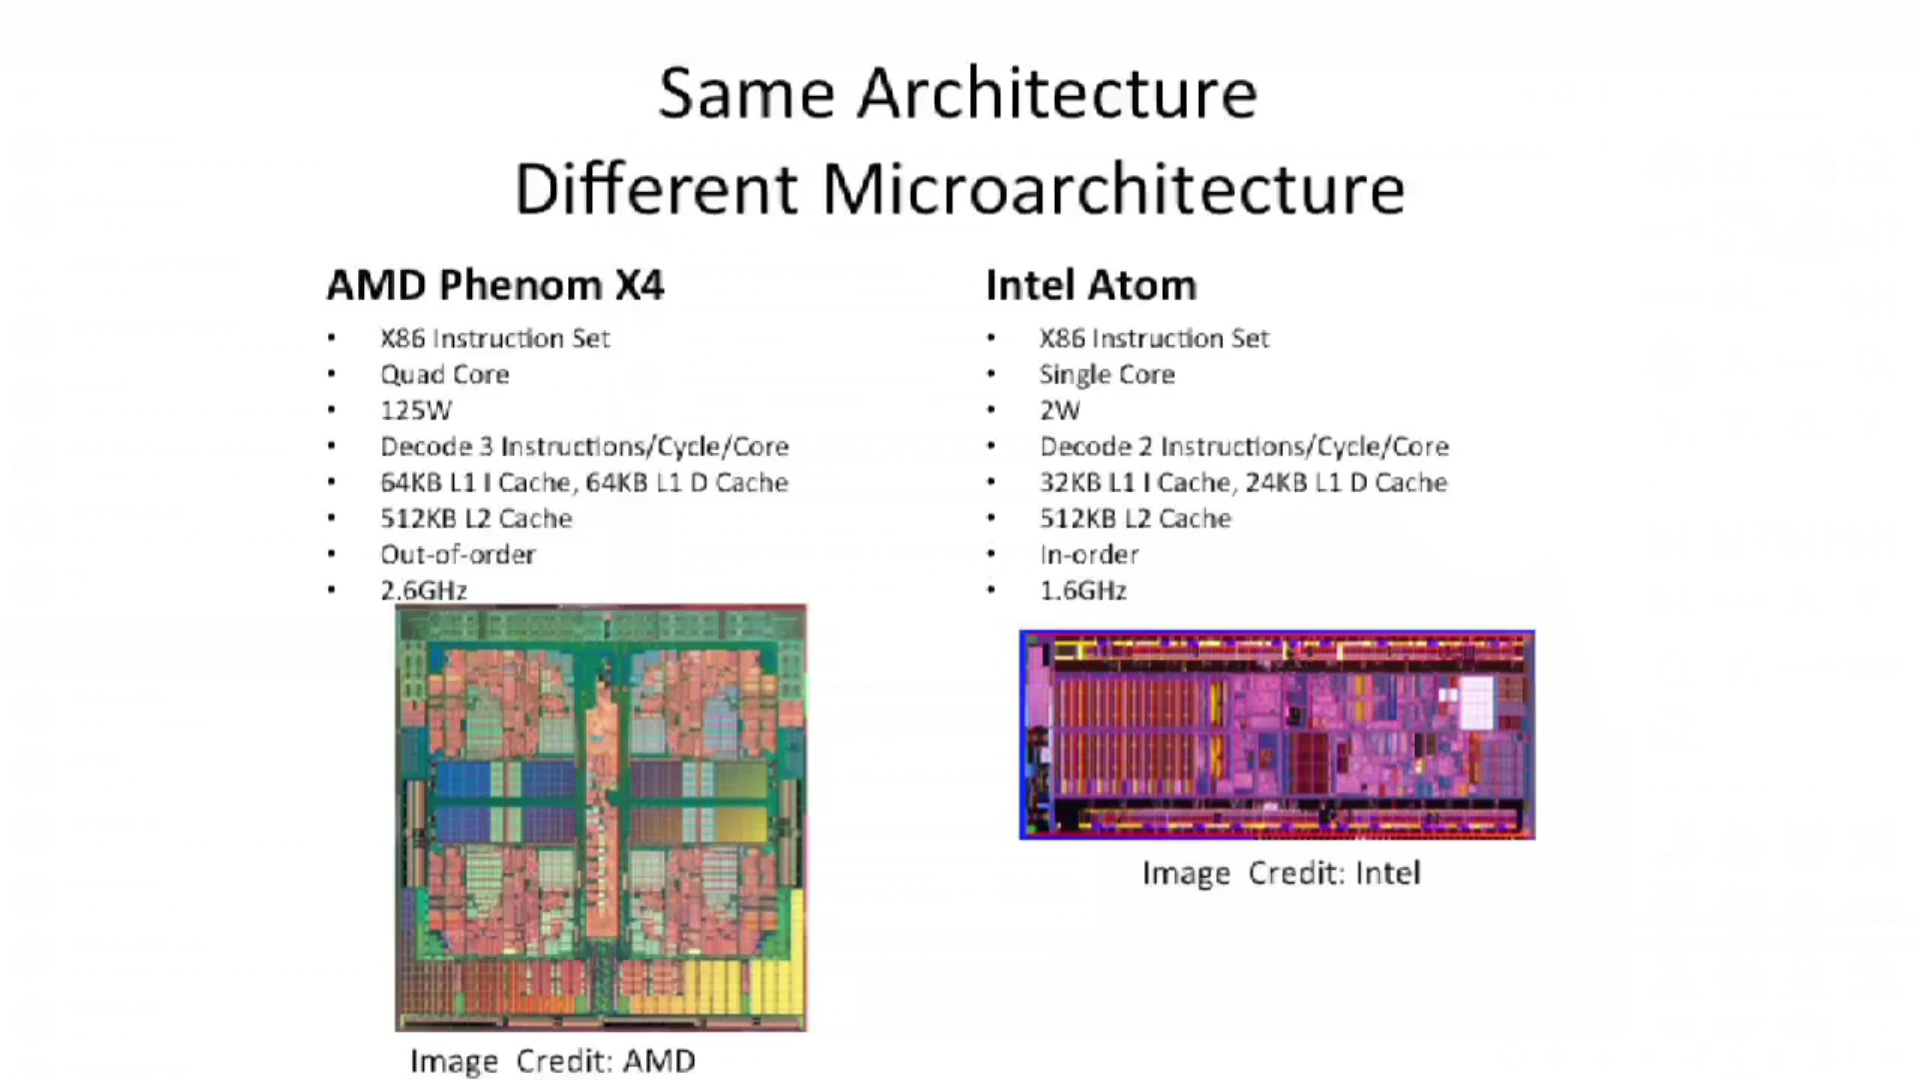
\includegraphics[width=0.8\linewidth]{./images/micro.png}
    \caption{}
    \label{fig:my_label}
\end{figure}
\end{document}